\section{Thiết kế class diagram}

Do thiết kế class diagram quá lớn không thể trình bày trên một trang tài liệu. Vì thế, tài liệu này phân tích thiết kế của class diagram thành những tập hợp các thành phần nhỏ của một số module có liên quan đến nhau cho luồng thực thi nghiệp vụ nào đó.

Thiết kế đầy đủ: \href{https://drive.google.com/file/d/17kk1Cg_yC6LihpOeuelwq7wTC-_Zbwdg/view?usp=sharing}{Thiết kế Class Diagram}
\subsection{Nghiệp vụ 1: Nhân viên thực hiện chọn món và tạo order}

\begin{figure}[H]
    \centering
    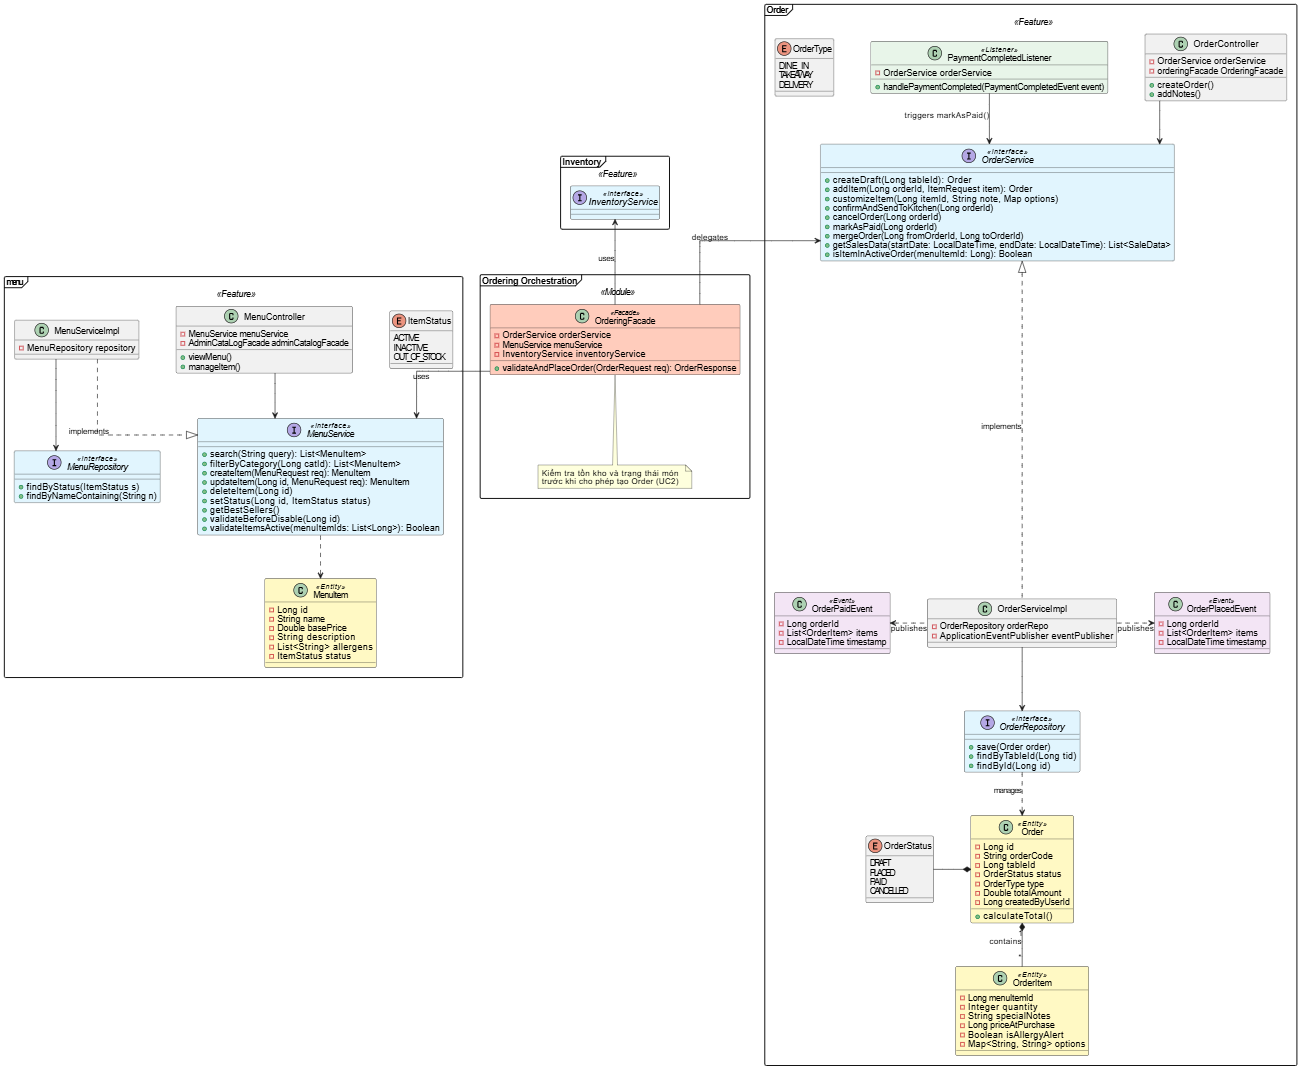
\includegraphics[width=0.9\textwidth]{./figs/class-diagram/class-diagram-uc-1-2-3.png}
    \caption{Thiết kế class diagram cho nghiệp vụ tạo order}
    \label{fig:myimage}
\end{figure}

\newpage

Khi thực thi các module trong hình sẽ có những tương tác phụ thuộc lẫn nhau như trong hình 1 với các API như sau:
\begin{itemize}
    \item \texttt{createDraft(Long tableId): Order}: trả về một order nháp được khởi tạo. Được gọi trong \texttt{createOrder} thuộc class \texttt{OrderController}.
    \item \texttt{addItem(Long orderId ItemRequest item): Order}: thực thi khi nhân viên thêm các món ăn vào một order vừa mới tạo.
    \item \texttt{customizeItem(Long itemId, String note, Map options)}: thực thi tạo một OrderItem bao gồm \textbf{note} (Lưu ý của khách hàng khi order), \textbf{options} (Những yêu cầu bổ sung như topping hay thêm cơm)
\end{itemize}

Bên cạnh đó, việc thực hiện logic kiểm tra và thực sự tạo một order trong hệ thống sẽ được kiểm tra và quyết định tạo order bởi module \textbf{OrderFacade} khác. Thiết kế này đảm bảo nguyên lý Single Responsibility trong SOLID, khi module Order không cần biết việc kiểm tra menuItem hợp lệ diễn ra thế nào. Ngoài ra, việc đặt code được hiện thực ra một module khác như vậy giúp dễ bảo trì logic kiểm tra trạng thái của một thực thể thuộc module khác.

\newpage

\subsection{Nghiệp vụ 2: Quản trị viên thiết lập Catalog (Menu và Khuyến mãi)}
\begin{figure}[H]
    \centering
    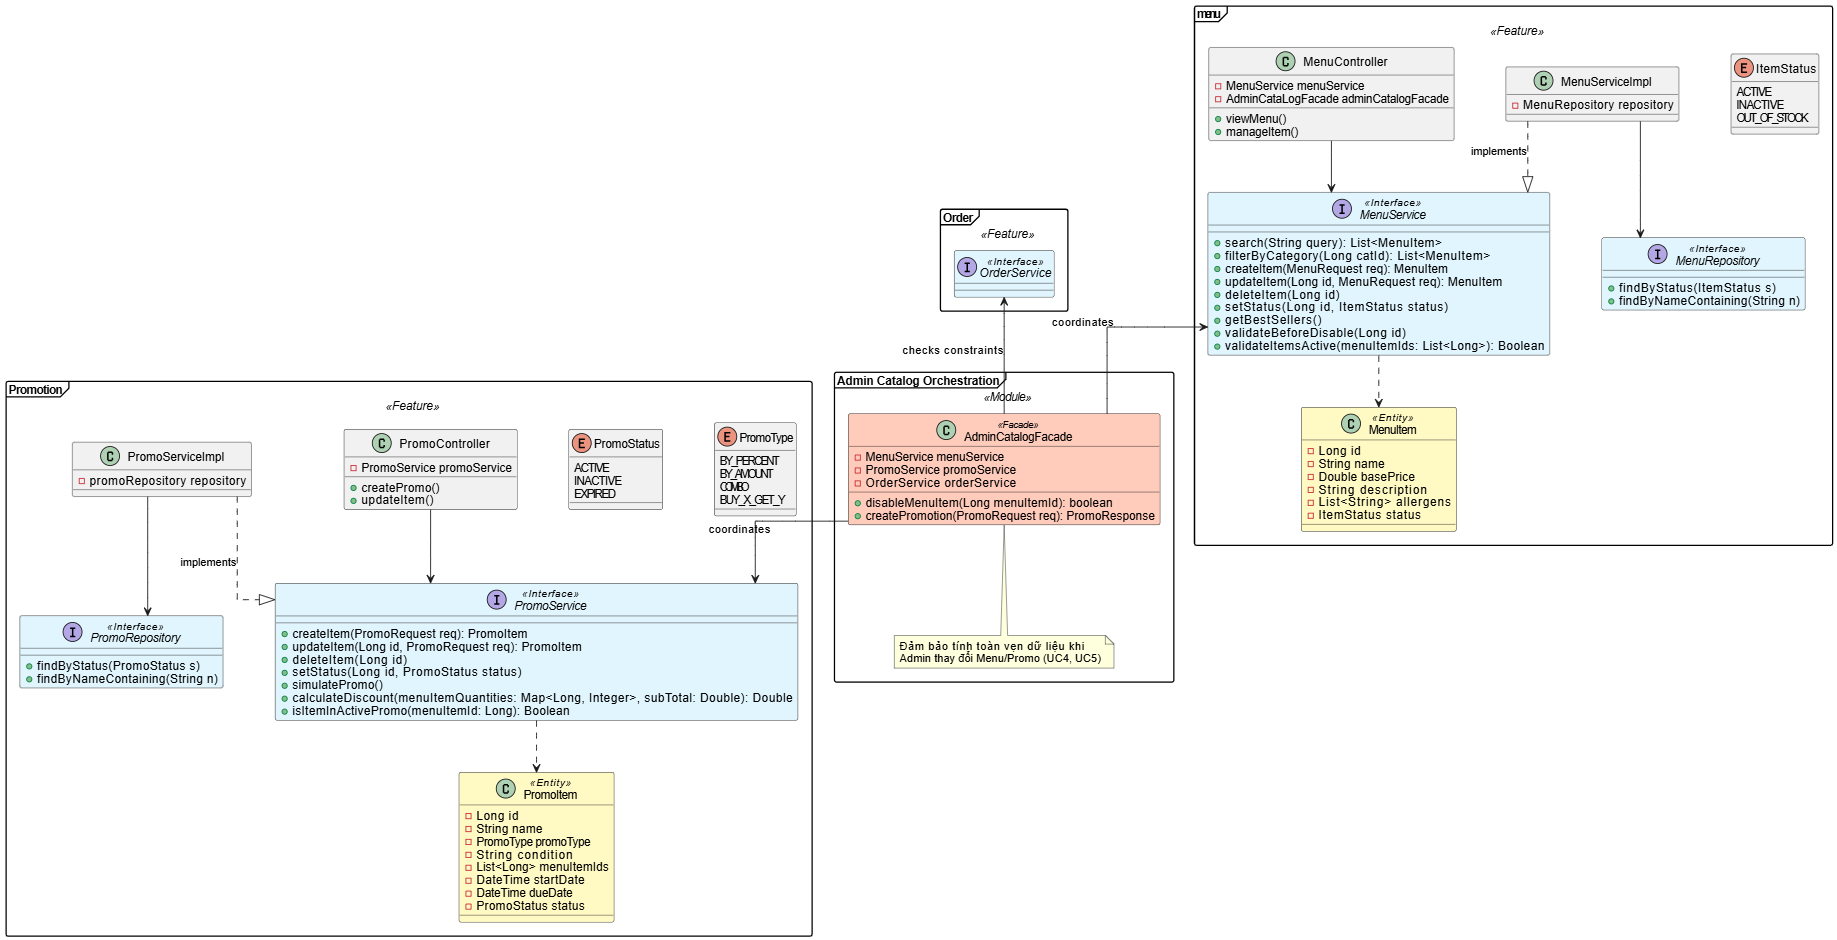
\includegraphics[width=0.9\textwidth]{./figs/class-diagram/class-diagram-uc-4-5.drawio.png}
    \caption{Thiết kế class diagram cho nghiệp vụ quản lý danh mục và khuyến mãi}
    \label{fig:admin_catalog}
\end{figure}
Nghiệp vụ quản lý thực đơn và các chương trình khuyến mãi đòi hỏi tính toàn vẹn dữ liệu cao giữa các phân hệ. Các API chính tham gia vào tiến trình này bao gồm:
\begin{itemize}
    \item \texttt{createItem(MenuRequest req): MenuItem} và \texttt{createItem(PromoRequest req): PromoItem}: tạo mới các thực thể món ăn hoặc chương trình khuyến mãi thông qua các Service tương ứng.
    \item \texttt{setStatus(Long id, ItemStatus status)}: thực hiện cập nhật trạng thái hoạt động của thực đơn (Active, Inactive, Out of Stock).
    \item \texttt{disableMenuItem(Long menuItemId): boolean}: API được bọc bởi \textbf{AdminCatalogFacade} để thực hiện vô hiệu hóa một món ăn một cách an toàn.
\end{itemize}
Để tránh việc dữ liệu bị lỗi (ví dụ: xóa một món ăn đang nằm trong một chương trình khuyến mãi đang chạy hoặc một order chưa thanh toán), hệ thống áp dụng \textbf{Facade Pattern} thông qua \texttt{AdminCatalogFacade}. Module này đóng vai trò điều phối, sẽ thực hiện gọi chéo sang \texttt{OrderService} và \texttt{PromoService} để xác thực các ràng buộc nghiệp vụ trước khi ra lệnh cho \texttt{MenuService} cập nhật cơ sở dữ liệu.
    
\newpage
\subsection{Nghiệp vụ 3: Xử lý nhà bếp và Tự động trừ tồn kho}
\begin{figure}[H]
    \centering
    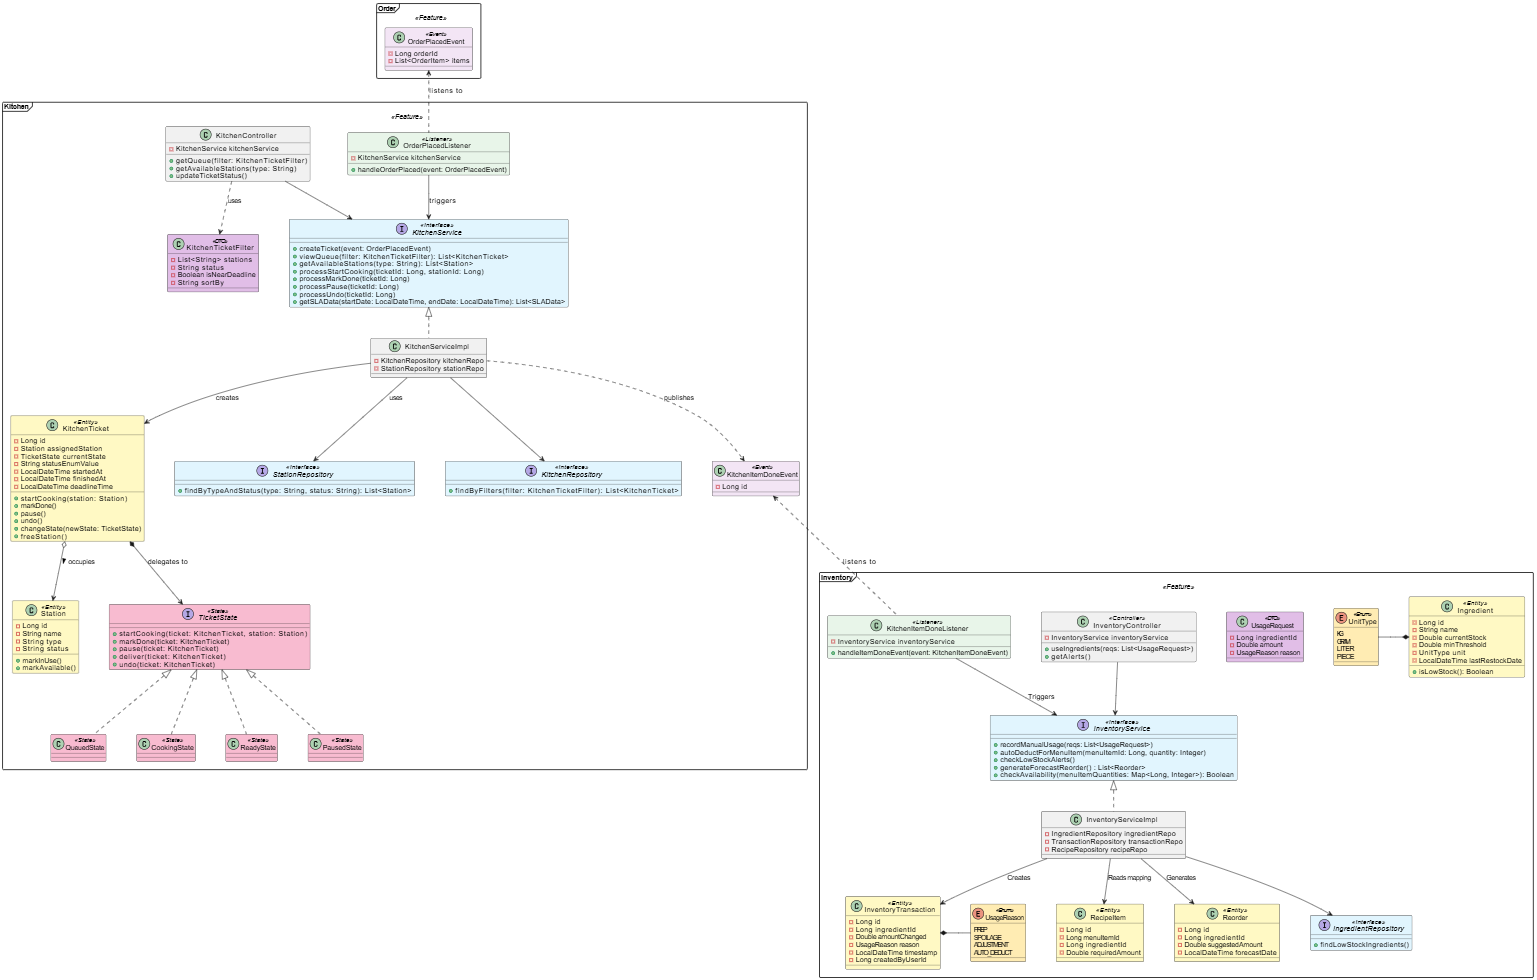
\includegraphics[width=0.9\textwidth]{./figs/class-diagram/class-diagram-uc-6-7-8-9-13.drawio.png}
    \caption{Thiết kế class diagram cho nghiệp vụ chế biến và quản lý nguyên liệu}
    \label{fig:kitchen_inventory}
\end{figure}
Đây là luồng nghiệp vụ hoạt động chủ yếu ngầm ở phía sau (Back of House), phụ thuộc mạnh vào cơ chế giao tiếp bất đồng bộ thông qua Event. Các API và hành vi chính bao gồm:
\begin{itemize}
    \item \texttt{handleOrderPlaced(event: OrderPlacedEvent)}: Listener phía Kitchen nhận tín hiệu từ luồng Order, sau đó gọi \texttt{createTicket} để tạo danh sách công việc cho đầu bếp.
    \item \texttt{changeState(newState: TicketState)}: quản lý vòng đời của một phiếu nấu ăn thông qua \textbf{State Pattern} (từ \texttt{QueuedState} sang \texttt{CookingState} và cuối cùng là \texttt{ReadyState}).
    \item \texttt{processMarkDone(ticketId: Long)}: Đầu bếp xác nhận hoàn thành món ăn. Hàm này sẽ phát ra sự kiện \texttt{KitchenItemDoneEvent}.
    \item \texttt{autoDeductForMenuItem(menuItemId: Long, quantity: Integer)}: Listener phía Inventory nhận sự kiện hoàn thành món, tra cứu \texttt{RecipeItem} để trừ nguyên liệu thô tự động.
\end{itemize}
Sự liên kết lỏng lẻo (loose coupling) ở đây mang lại lợi ích: các thao tác của nhà bếp hoàn toàn độc lập với kho. Sự tách biệt module và sử dụng \textbf{Observer Pattern} để giao tiếp giúp code dễ maintain theo từng module cũng như giảm sự phụ thuộc trong luồng thực thi giữa cả 2 module.
\newpage
\subsection{Nghiệp vụ 4: Thanh toán hóa đơn và Quản lý trạng thái bàn}
\begin{figure}[H]
    \centering
    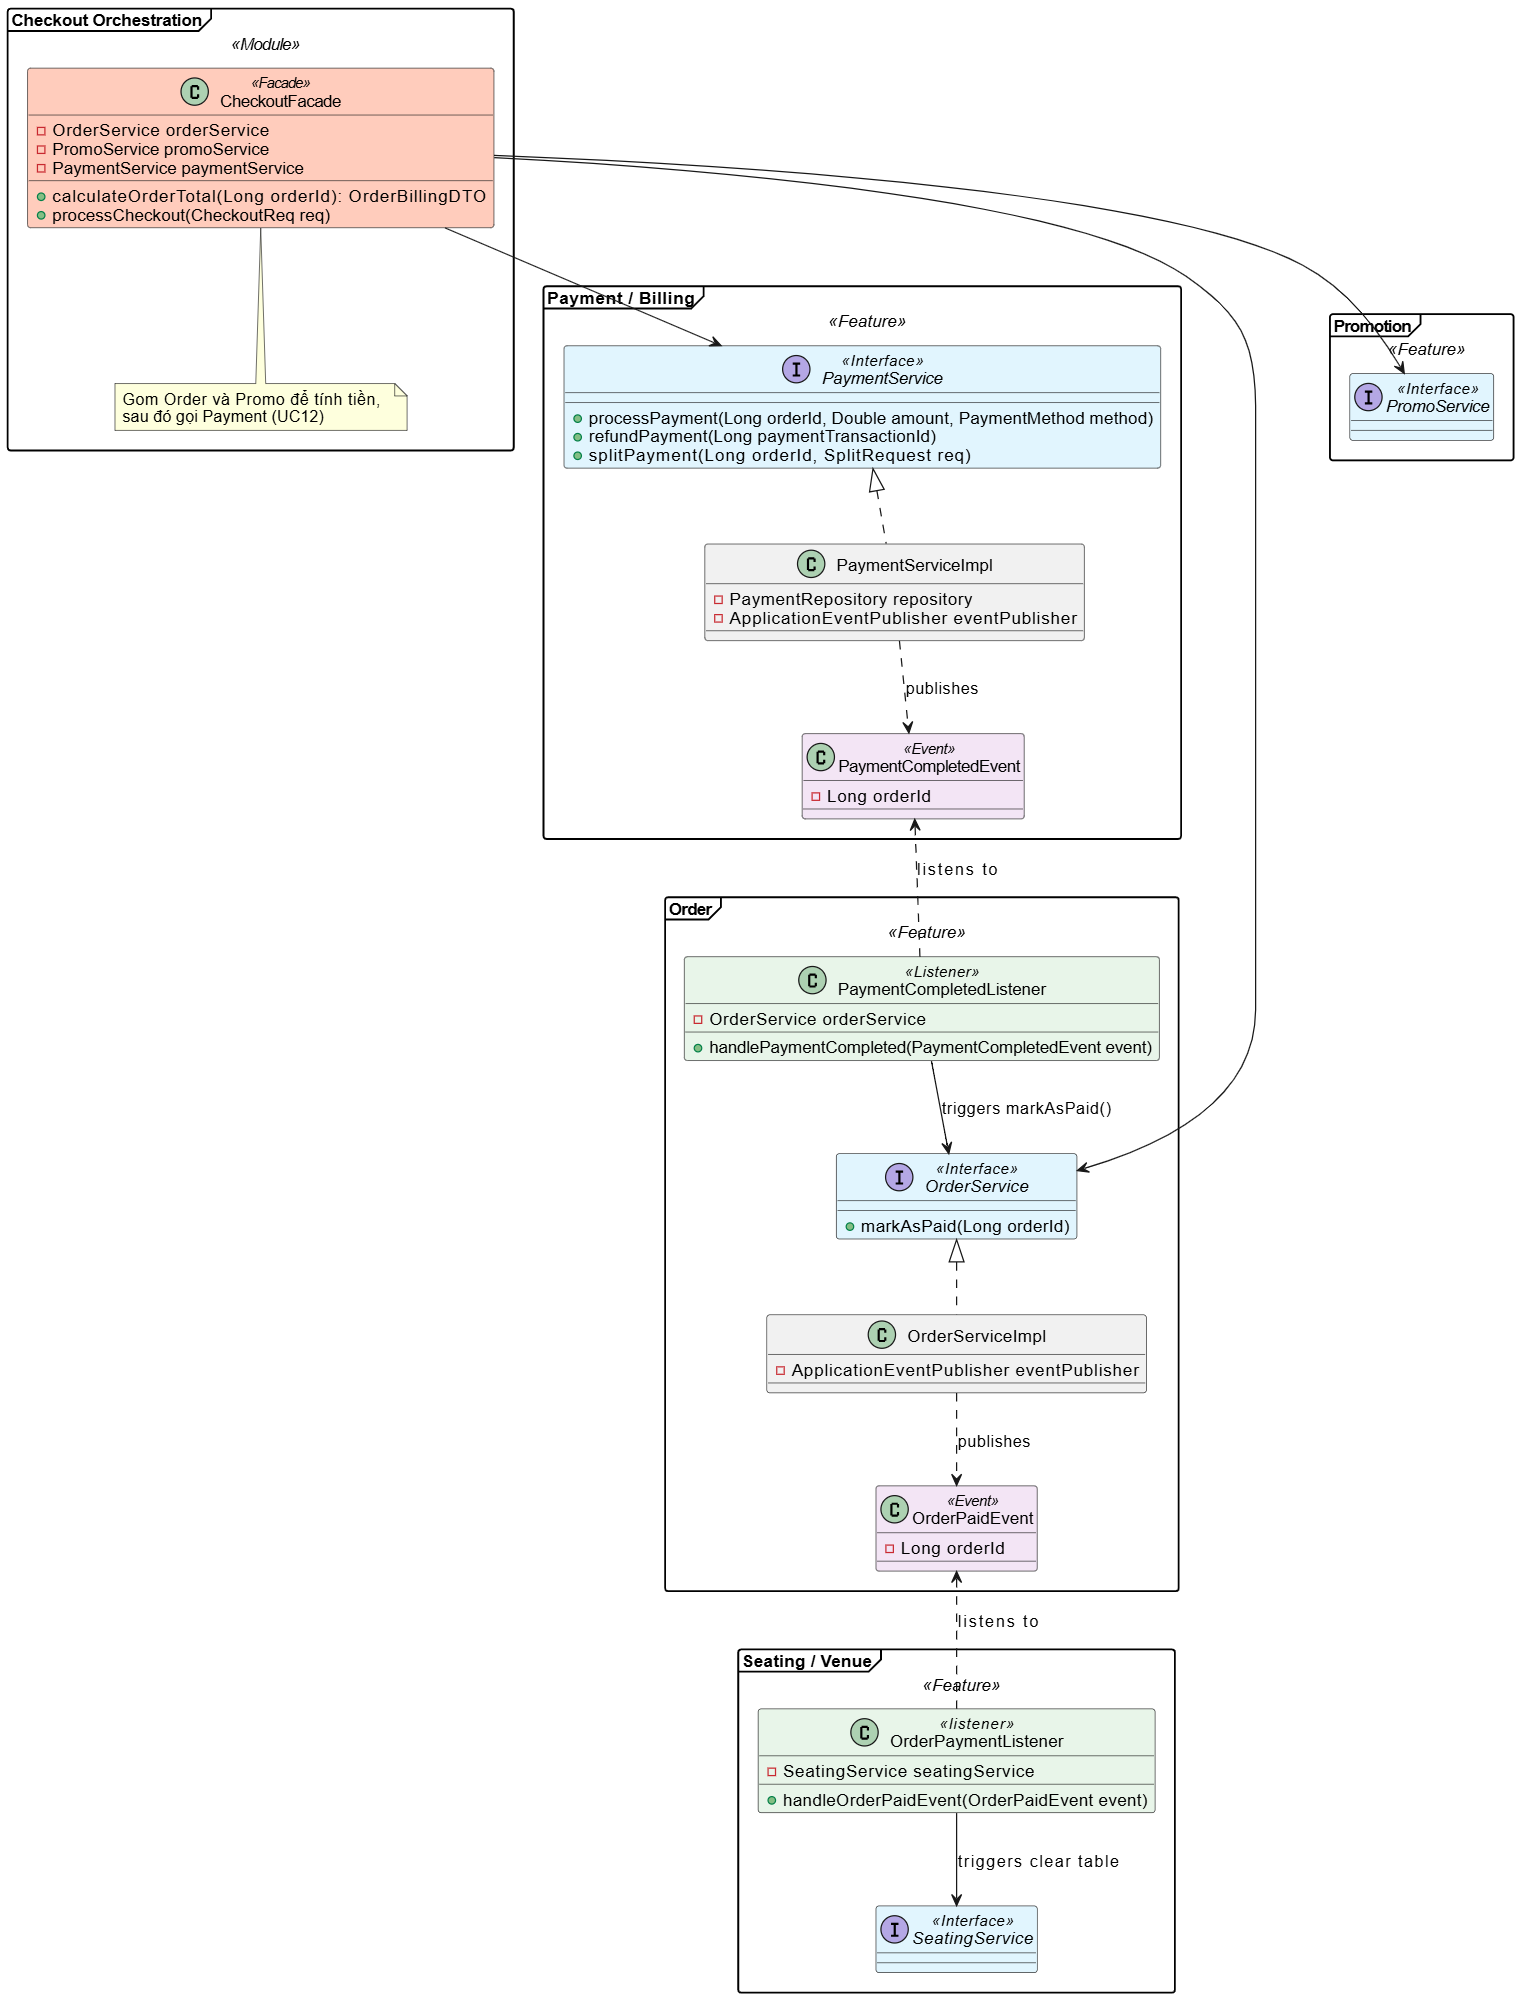
\includegraphics[width=0.9\textwidth]{./figs/class-diagram/class-diagram-uc-10-11-12.drawio.png}
    \caption{Thiết kế class diagram cho nghiệp vụ thanh toán và giải phóng bàn}
    \label{fig:checkout_seating}
\end{figure}
Giai đoạn cuối cùng của chu trình phục vụ khách hàng bao gồm việc tính toán chi phí, xử lý thanh toán và cập nhật sơ đồ nhà hàng.
\begin{itemize}
    \item \texttt{calculateOrderTotal(Long orderId)}: được gọi qua \texttt{CheckoutFacade} nhằm gom dữ liệu từ \texttt{OrderService} và tính toán mức giảm giá thông qua \texttt{PromoService}.
    \item \texttt{processPayment(Long orderId, Double amount, PaymentMethod method)}: thực thi giao dịch thanh toán và phát ra \texttt{PaymentCompletedEvent} khi thành công.
    \item \texttt{markAsPaid(Long orderId)}: \texttt{OrderService} lắng nghe giao dịch thành công để cập nhật trạng thái hóa đơn và tiếp tục kích hoạt \texttt{OrderPaidEvent}.
    \item \texttt{markAsDirty()}: API thuộc \texttt{Table} entity, được trigger bởi \texttt{OrderPaymentListener} thuộc module Seating để tự động báo cho nhân viên dọn bàn.
\end{itemize}
Việc áp dụng \texttt{CheckoutFacade} giúp hệ thống giấu đi sự phức tạp của việc tính toán giá trị hóa đơn (bao gồm thuế, tip, khuyến mãi chồng chéo). Đồng thời, phản ứng dây chuyền qua Event (Payment $\rightarrow$ Order $\rightarrow$ Seating) đảm bảo sơ đồ nhà hàng (Floor plan) giúp tạo ra giao tiếp tự động giữa các module.
\newpage

\subsection{Nghiệp vụ 5: Phân tích dữ liệu và Xuất báo cáo}
\begin{figure}[H]
    \centering
    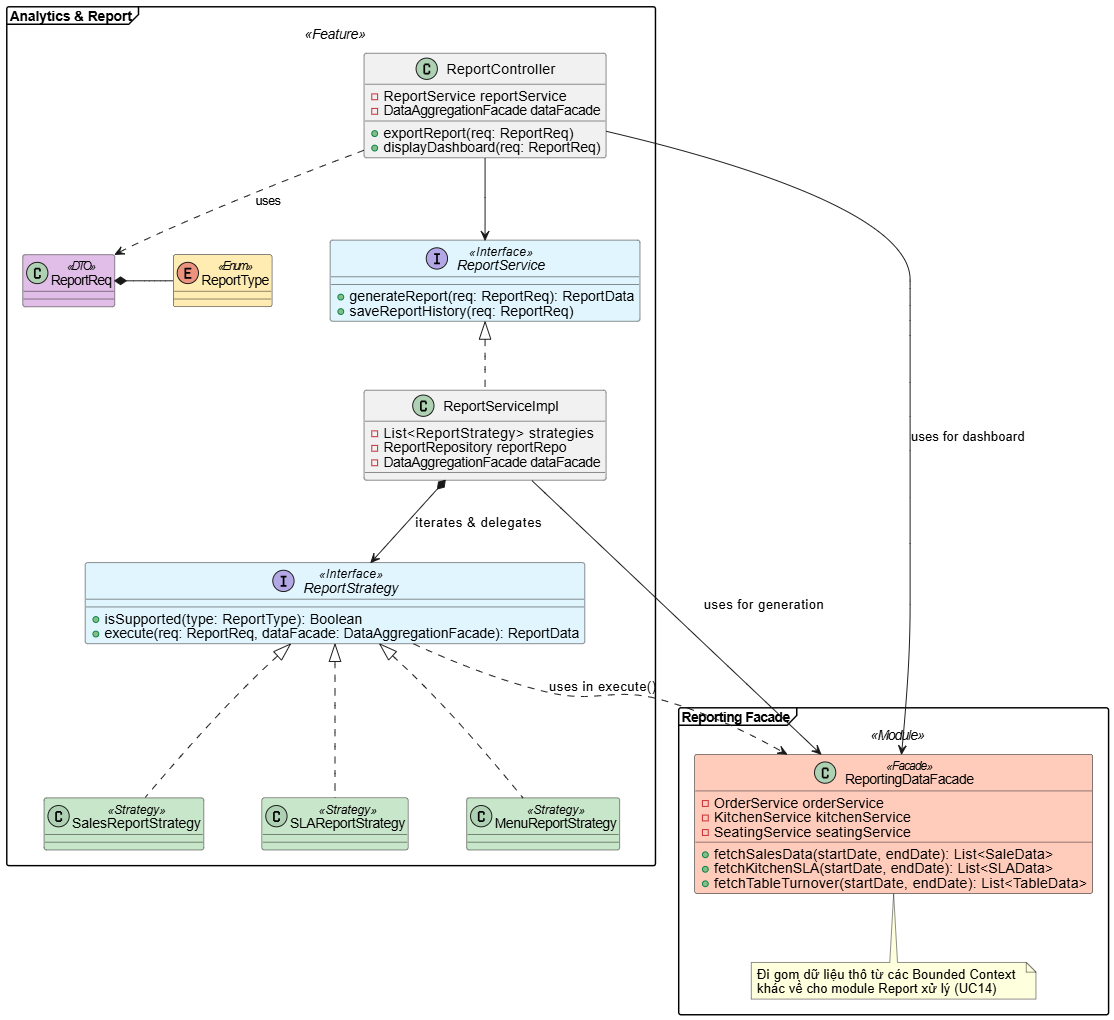
\includegraphics[width=0.9\textwidth]{./figs/class-diagram/class-diagram-uc-14.drawio.png}
    \caption{Thiết kế class diagram cho nghiệp vụ phân tích và tổng hợp báo cáo}
    \label{fig:analytics_reporting}
\end{figure}
Module Analytics hoạt động độc lập và không can thiệp vào tiến trình giao dịch của các phân hệ khác (Non-blocking).
\begin{itemize}
    \item \texttt{generateReport(req: ReportReq): ReportData}: điểm vào duy nhất cho mọi yêu cầu báo cáo.
    \item \texttt{execute(req, dataFacade)}: phương thức thuộc giao diện \texttt{ReportStrategy}. Tùy thuộc vào loại báo cáo, hệ thống sẽ gọi \texttt{SalesReportStrategy}, \texttt{SLAReportStrategy} hoặc \texttt{MenuReportStrategy}.
    \item \texttt{fetchSalesData}, \texttt{fetchKitchenSLA}: Các API gom dữ liệu thô từ các module nghiệp vụ khác thông qua \texttt{ReportingDataFacade}.
\end{itemize}
Thiết kế kết hợp giữa \textbf{Strategy Pattern} và \textbf{Facade Pattern} giúp hệ thống Report dễ dàng mở rộng. Khi nhà hàng cần thêm một loại báo cáo mới (ví dụ: Báo cáo nhân sự), ta chỉ cần tạo thêm một Strategy class mới mà không làm ảnh hưởng đến mã nguồn cũ (tuân thủ nguyên lý Open/Closed trong SOLID).
\newpage
\subsection{Nghiệp vụ 6: Kiểm soát truy cập và Lưu vết hệ thống (Cross-Cutting)}
\begin{figure}[H]
    \centering
    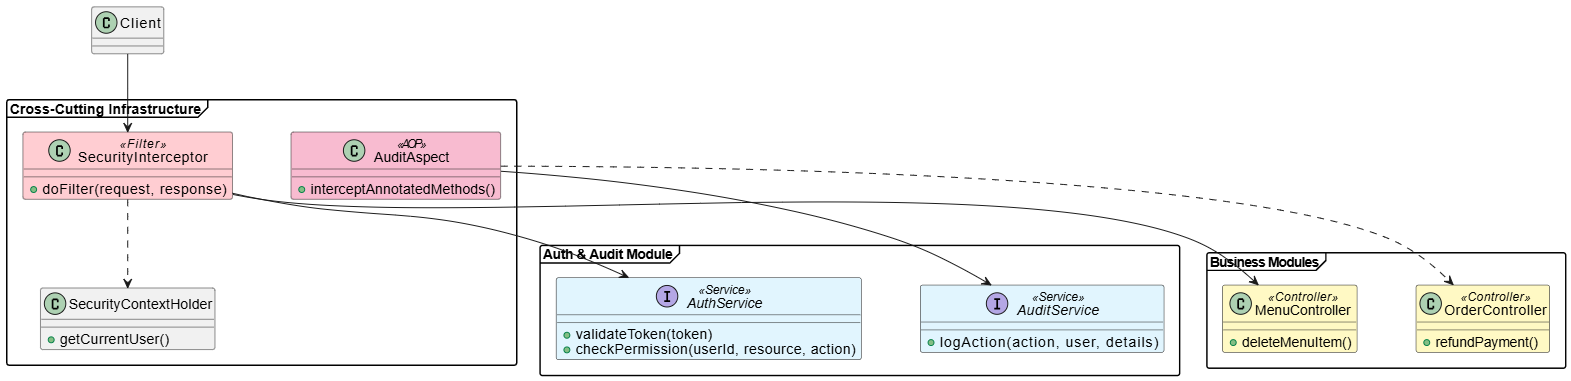
\includegraphics[width=0.9\textwidth]{./figs/class-diagram/class-diagram-uc-15.drawio.png}
    \caption{Thiết kế class diagram cho hạ tầng phân quyền và Audit}
    \label{fig:security_audit}
\end{figure}
Để đảm bảo tính bảo mật và truy vết (đặc biệt trong các thao tác nhạy cảm như hoàn tiền, xóa món), hệ thống áp dụng kiến trúc Cross-Cutting Concerns.
\begin{itemize}
    \item \texttt{doFilter(request, response)}: Thuộc \texttt{SecurityInterceptor}, chặn mọi luồng API đi vào hệ thống để xác thực Token và kiểm tra vai trò người dùng qua \texttt{AuthService}.
    \item \texttt{interceptAnnotatedMethods()}: Thuộc \texttt{AuditAspect}, tự động bao bọc các Controller nhạy cảm.
    \item \texttt{logAction(action, user, details)}: Ghi nhận lịch sử thao tác vào cơ sở dữ liệu.
\end{itemize}
Việc sử dụng \textbf{AOP (Aspect-Oriented Programming)} thông qua \texttt{AuditAspect} là một thiết kế tối ưu. Nó giúp bóc tách hoàn toàn logic kiểm tra quyền và ghi log ra khỏi logic nghiệp vụ chính (Business Logic) bên trong các Service. Nhờ đó, mã nguồn của \texttt{OrderController} hay \texttt{MenuController} giữ được sự gọn gàng và dễ đọc.